%% BioMed_Central_Tex_Template_v1.06
%%                                      %
%  bmc_article.tex            ver: 1.06 %
%                                       %

%%IMPORTANT: do not delete the first line of this template
%%It must be present to enable the BMC Submission system to
%%recognise this template!!

%%%%%%%%%%%%%%%%%%%%%%%%%%%%%%%%%%%%%%%%%
%%                                     %%
%%  LaTeX template for BioMed Central  %%
%%     journal article submissions     %%
%%                                     %%
%%          <8 June 2012>              %%
%%                                     %%
%%                                     %%
%%%%%%%%%%%%%%%%%%%%%%%%%%%%%%%%%%%%%%%%%


%%%%%%%%%%%%%%%%%%%%%%%%%%%%%%%%%%%%%%%%%%%%%%%%%%%%%%%%%%%%%%%%%%%%%
%%                                                                 %%
%% For instructions on how to fill out this Tex template           %%
%% document please refer to Readme.html and the instructions for   %%
%% authors page on the biomed central website                      %%
%% http://www.biomedcentral.com/info/authors/                      %%
%%                                                                 %%
%% Please do not use \input{...} to include other tex files.       %%
%% Submit your LaTeX manuscript as one .tex document.              %%
%%                                                                 %%
%% All additional figures and files should be attached             %%
%% separately and not embedded in the \TeX\ document itself.       %%
%%                                                                 %%
%% BioMed Central currently use the MikTex distribution of         %%
%% TeX for Windows) of TeX and LaTeX.  This is available from      %%
%% http://www.miktex.org                                           %%
%%                                                                 %%
%%%%%%%%%%%%%%%%%%%%%%%%%%%%%%%%%%%%%%%%%%%%%%%%%%%%%%%%%%%%%%%%%%%%%

%%% additional documentclass options:
%  [doublespacing]
%  [linenumbers]   - put the line numbers on margins

%%% loading packages, author definitions

%\documentclass[twocolumn]{bmcart}% uncomment this for twocolumn layout and comment line below
\documentclass{bmcart}

%%% Load packages
%\usepackage{amsthm,amsmath}
%\RequirePackage{natbib}
%\RequirePackage[authoryear]{natbib}% uncomment this for author-year bibliography
%\RequirePackage{hyperref}
\usepackage[utf8]{inputenc} %unicode support
%\usepackage[applemac]{inputenc} %applemac support if unicode package fails
%\usepackage[latin1]{inputenc} %UNIX support if unicode package fails
\usepackage{graphicx}
\usepackage{booktabs}
\usepackage{amsfonts}
\usepackage{subfig}
\usepackage[ruled,lined]{algorithm2e}
\usepackage{multirow}
\usepackage{color}
\usepackage{flushend}
\usepackage[bookmarks=false]{hyperref}
\usepackage{setspace} % for setstretch in algorithm
\usepackage{amssymb, amsmath}
\usepackage{xspace}


%%%%%%%%%%%%%%%%%%%%%%%%%%%%%%%%%%%%%%%%%%%%%%%%%
%%                                             %%
%%  If you wish to display your graphics for   %%
%%  your own use using includegraphic or       %%
%%  includegraphics, then comment out the      %%
%%  following two lines of code.               %%
%%  NB: These line *must* be included when     %%
%%  submitting to BMC.                         %%
%%  All figure files must be submitted as      %%
%%  separate graphics through the BMC          %%
%%  submission process, not included in the    %%
%%  submitted article.                         %%
%%                                             %%
%%%%%%%%%%%%%%%%%%%%%%%%%%%%%%%%%%%%%%%%%%%%%%%%%


%%% Put your definitions there:
\startlocaldefs
\endlocaldefs

\newcommand{\red}[1]{\textcolor{red}{#1}}
\newcommand{\tylde}{$\sim$}

%\hypersetup{colorlinks=true,linkcolor=black,citecolor=black}

\SetKwInput{KwData}{Global params.}

\def\qrand{q_{rand}}
\def\qstart{q_{start}}
\def\qinit{\qstart}
\def\qgoal{q_{goal}}
\def\qnear{q_{near}}
\def\qnew{q_{new}}
\def\T{\mathcal{T}}

\def\C{\mathcal{C}}
\def\CF{\mathcal{C}_{free}}
\def\dtg{d_{t}}
%\def\da{d_{atom}}
\def\dist{\varrho}
\def\distt{\varrho_{3D}}
\def\R{\mathbb{R}}

\def\rv{R_{tunnel}}


\def\Imax{I_{max}} %max number of iterations of RRT-based planners

\def\dist{\mathrm{dist}}
\def\dists{\mathrm{dist}_{\mathrm{s}}}

\SetKw{return}{return}

\def\sdelta{s_{\Delta}}


\def\probe{r_{\mathrm{probe}}}
\def\Sprobe{S_{\mathrm{probe}}}

\def\gprobe{r_{\mathrm{out}}}
\def\Sgprobe{S_{\mathrm{out}}}


\def\CG{\mathcal{C}_{goal}}
\def\SB{\mathbf{S}_{blocking}}
\def\SS{\mathbf{S}}


%spacing for algorithm environment. 1.0 mean normal spacing
\def\gb{p_{tunnel}}

\def\L{\mathcal{L}}
\def\S{\mathcal{S}}

\def\LA{L_1}
\def\LB{L_2}

\def\RA{A$_{1}$}
\def\RB{A$_{2}$}
\def\RC{A$_{1}^{*}$}
\def\RD{A$_1^P$}

%%% Begin ...
\begin{document}

%%% Start of article front matter
\begin{frontmatter}

\begin{fmbox}
\dochead{Research}

%%%%%%%%%%%%%%%%%%%%%%%%%%%%%%%%%%%%%%%%%%%%%%
%%                                          %%
%% Enter the title of your article here     %%
%%                                          %%
%%%%%%%%%%%%%%%%%%%%%%%%%%%%%%%%%%%%%%%%%%%%%%

\title{Motion Planning for Assessing the Accessibility of Protein Tunnels}

%%%%%%%%%%%%%%%%%%%%%%%%%%%%%%%%%%%%%%%%%%%%%%
%%                                          %%
%% Enter the authors here                   %%
%%                                          %%
%% Specify information, if available,       %%
%% in the form:                             %%
%%   <key>={<id1>,<id2>}                    %%
%%   <key>=                                 %%
%% Comment or delete the keys which are     %%
%% not used. Repeat \author command as much %%
%% as required.                             %%
%%                                          %%
%%%%%%%%%%%%%%%%%%%%%%%%%%%%%%%%%%%%%%%%%%%%%%

\author[
   addressref={aff1},                   % id's of addresses, e.g. {aff1,aff2}
   corref={aff1},                       % id of corresponding address, if any
  % noteref={n1},                        % id's of article notes, if any
   email={vonasek@labe.felk.cvut.cz}   % email address
]{\inits{VV}\fnm{Vojt\v ech} \snm{Von\' asek}}
\author[
   addressref={aff2},
   %email={john.RS.Smith@cambridge.co.uk}
]{\inits{BK}\fnm{Barbora} \snm{Kozl\'\i kov\'a}}
\author[
   addressref={aff2},
   %email={john.RS.Smith@cambridge.co.uk}
]{\inits{AJ}\fnm{Adam} \snm{Jur\v{c}\'\i k}}
\author[
   addressref={aff3},
   %email={john.RS.Smith@cambridge.co.uk}
]{\inits{OV}\fnm{Ond\v{r}ej} \snm{V\'{a}vra}}
\author[
   addressref={aff1},
   %email={john.RS.Smith@cambridge.co.uk}
]{\inits{MS}\fnm{Martin} \snm{Saska}}


%%%%%%%%%%%%%%%%%%%%%%%%%%%%%%%%%%%%%%%%%%%%%%
%%                                          %%
%% Enter the authors' addresses here        %%
%%                                          %%
%% Repeat \address commands as much as      %%
%% required.                                %%
%%                                          %%
%%%%%%%%%%%%%%%%%%%%%%%%%%%%%%%%%%%%%%%%%%%%%%

\address[id=aff1]{%                           % unique id
  \orgname{Faculty of Electrical Engineering,  Czech Technical University in Prague}, % university, etc
  \street{Technick\'a 2},                     %
  %\postcode{}                                % post or zip code
  \city{Prague},                              % city
  \cny{Czech Republic}                                    % country
}
\address[id=aff2]{%
  \orgname{Faculty of Informatics, Masaryk University},
  \street{Botanick\'a 68a},
  %\postcode{24105}
  \city{Brno},
  \cny{Czech Republic}
}
\address[id=aff3]{%
  \orgname{Loschmidt Laboratories, Department of Experimental Biology RECETOX, Faculty of Science, Masaryk University},
  \street{Kamenice 5},
  %\postcode{24105}
  \city{Brno},
  \cny{Czech Republic}
}
%%%%%%%%%%%%%%%%%%%%%%%%%%%%%%%%%%%%%%%%%%%%%%
%%                                          %%
%% Enter short notes here                   %%
%%                                          %%
%% Short notes will be after addresses      %%
%% on first page.                           %%
%%                                          %%
%%%%%%%%%%%%%%%%%%%%%%%%%%%%%%%%%%%%%%%%%%%%%%

%\begin{artnotes}
%\note{Sample of title note}     % note to the article
%\note[id=n1]{Equal contributor} % note, connected to author
%\end{artnotes}

\end{fmbox}% comment this for two column layout

%%%%%%%%%%%%%%%%%%%%%%%%%%%%%%%%%%%%%%%%%%%%%%
%%                                          %%
%% The Abstract begins here                 %%
%%                                          %%
%% Please refer to the Instructions for     %%
%% authors on http://www.biomedcentral.com  %%
%% and include the section headings         %%
%% accordingly for your article type.       %%
%%                                          %%
%%%%%%%%%%%%%%%%%%%%%%%%%%%%%%%%%%%%%%%%%%%%%%


\begin{abstractbox}

\begin{abstract} % abstract
\parttitle{Background} %if any
Chemical interactions between proteins and other molecules (ligands) take place in specific locations, called active sites, that are often deeply buried inside the protein structure.
These active sites are accessible through one or more void paths, called tunnels.
Nowadays, tunnels are mostly computed using Voronoi diagrams which approximate the ligand by a bounding sphere and 
the traversability of the tunnels is determined based only on the radial bottlenecks.
This can lead to imprecise results as the shape of the ligand is not considered.

\parttitle{Results} %if any
We propose a method to compute trajectories of ligands along selected tunnels in the proteins.
The trajectories are computed using a novel motion planner based on Rapidly Exploring Random Tress, that searches
the corresponding configuration space.
The flexibility of the ligand is modeled by alowing rotations of the dihedral angles.
The search of the trajectories is guided using the information of the spherial tunnels.
By constraining the search to the vicinity of the tunnels, trajectories can be found significnatly faster than with other related tools.
The resulted trajectories are evaluted using an energy  profile, which enables chemists to revelan new information about the tunnels and
help to decide if the analyzed tunnels are accessible for the ligands being tested.

\parttitle{Conclusions} %if any
The proposed method has been evaluated in a virtual screening scenario to estimate the traversability of tunnels for several ligands.
\end{abstract}

%%%%%%%%%%%%%%%%%%%%%%%%%%%%%%%%%%%%%%%%%%%%%%
%%                                          %%
%% The keywords begin here                  %%
%%                                          %%
%% Put each keyword in separate \kwd{}.     %%
%%                                          %%
%%%%%%%%%%%%%%%%%%%%%%%%%%%%%%%%%%%%%%%%%%%%%%

\begin{keyword}
\kwd{protein}
\kwd{tunnel}
\kwd{motion planning}
\end{keyword}

% MSC classifications codes, if any
%\begin{keyword}[class=AMS]
%\kwd[Primary ]{}
%\kwd{}
%\kwd[; secondary ]{}
%\end{keyword}

\end{abstractbox}
%
%\end{fmbox}% uncomment this for twcolumn layout

\end{frontmatter}

%%%%%%%%%%%%%%%%%%%%%%%%%%%%%%%%%%%%%%%%%%%%%%
%%                                          %%
%% The Main Body begins here                %%
%%                                          %%
%% Please refer to the instructions for     %%
%% authors on:                              %%
%% http://www.biomedcentral.com/info/authors%%
%% and include the section headings         %%
%% accordingly for your article type.       %%
%%                                          %%
%% See the Results and Discussion section   %%
%% for details on how to create sub-sections%%
%%                                          %%
%% use \cite{...} to cite references        %%
%%  \cite{koon} and                         %%
%%  \cite{oreg,khar,zvai,xjon,schn,pond}    %%
%%  \nocite{smith,marg,hunn,advi,koha,mouse}%%
%%                                          %%
%%%%%%%%%%%%%%%%%%%%%%%%%%%%%%%%%%%%%%%%%%%%%%

%%%%%%%%%%%%%%%%%%%%%%%%% start of article main body
% <put your article body there>

%%%%%%%%%%%%%%%%
%% Background %%
%%
\section*{Background}

{\color{red}TODO add ref \cite{zhou2010gates}}

The reactivity of proteins with other molecules plays a crucial role in many research disciplines, including protein engineering and drug design.
Protein reactivity is tightly connected with the presence of the void space between its amino acids. 
This space, forming a path called a tunnel, can be utilized by a small molecule (ligand) which can enter the protein inner space and react with the amino acids surrounding the protein active site~\cite{gora2013gates,marques2017enzyme} (see Fig.~\ref{fig::motiv}).
The location and size of a tunnel determine the size and shape of a ligand passing through this tunnel to the active site.
Currently, the biochemists can use various computational methods for tunnel detection in order to estimate the possibility of interactions between the protein and ligand.
This can help them to reduce the number of necessary in-vitro experiments.
The most common tools detect the tunnels using Voronoi diagrams~\cite{yaffe2008,caver3}, assuming a spherical ligand (probe), 
i.e., they approximate the ligand by a bounding sphere.
However, ligands are typically of a non-spherical shape, which is completely ignored by these methods. 

\begin{figure}[t]
\centering
{\footnotesize
\renewcommand{\arraystretch}{-0.5}
\renewcommand{\tabcolsep}{-1pt}
\begin{tabular}{ccc}
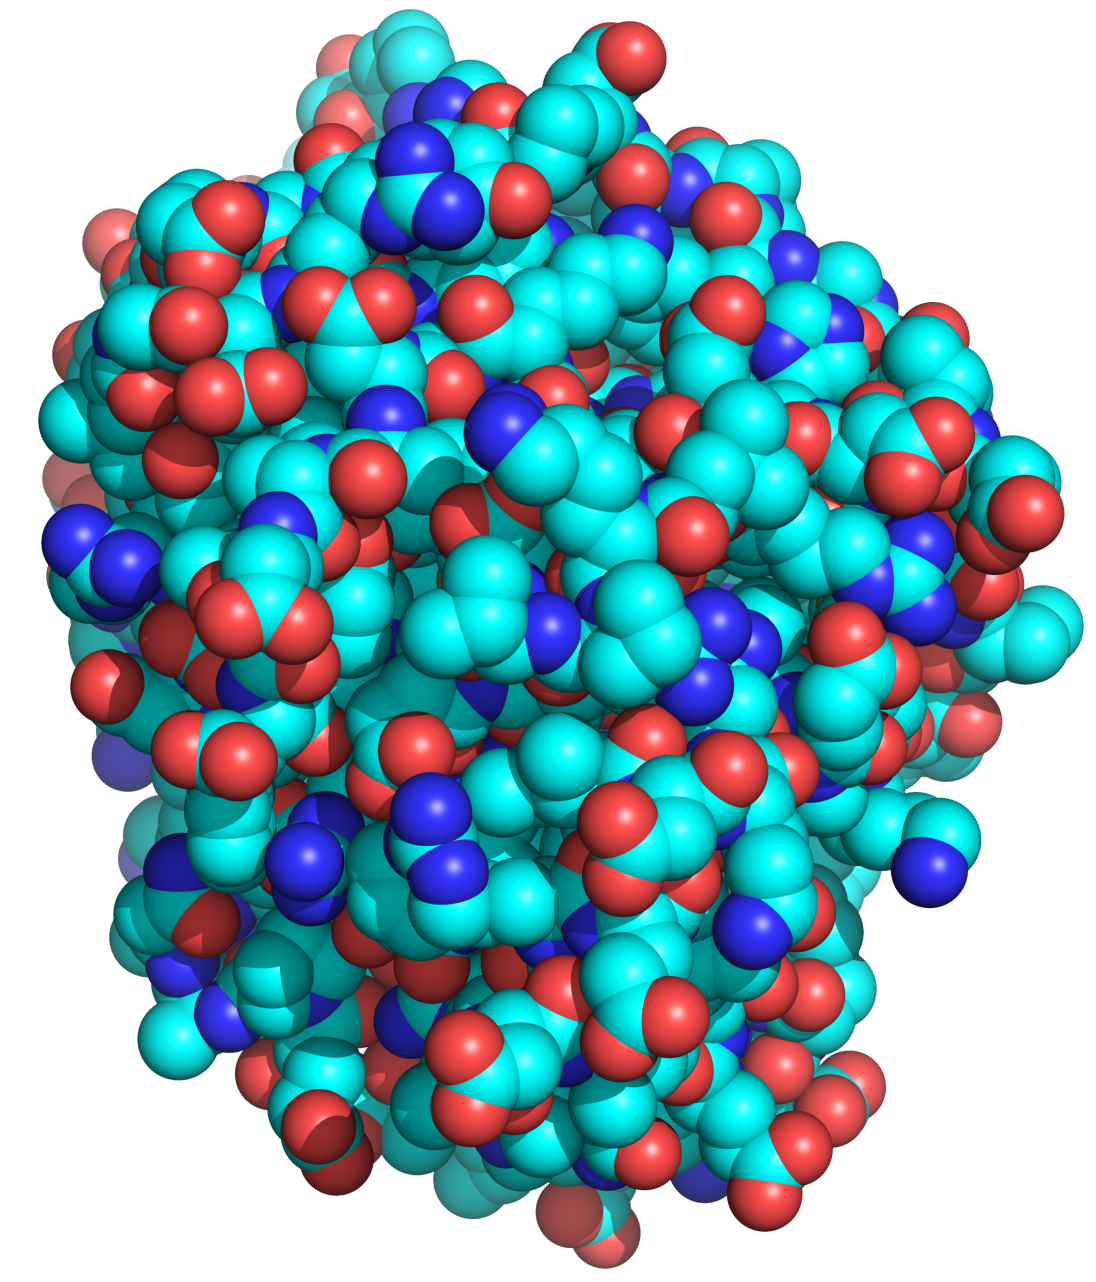
\includegraphics[width=0.24\textwidth]
{fig/motiv1} &
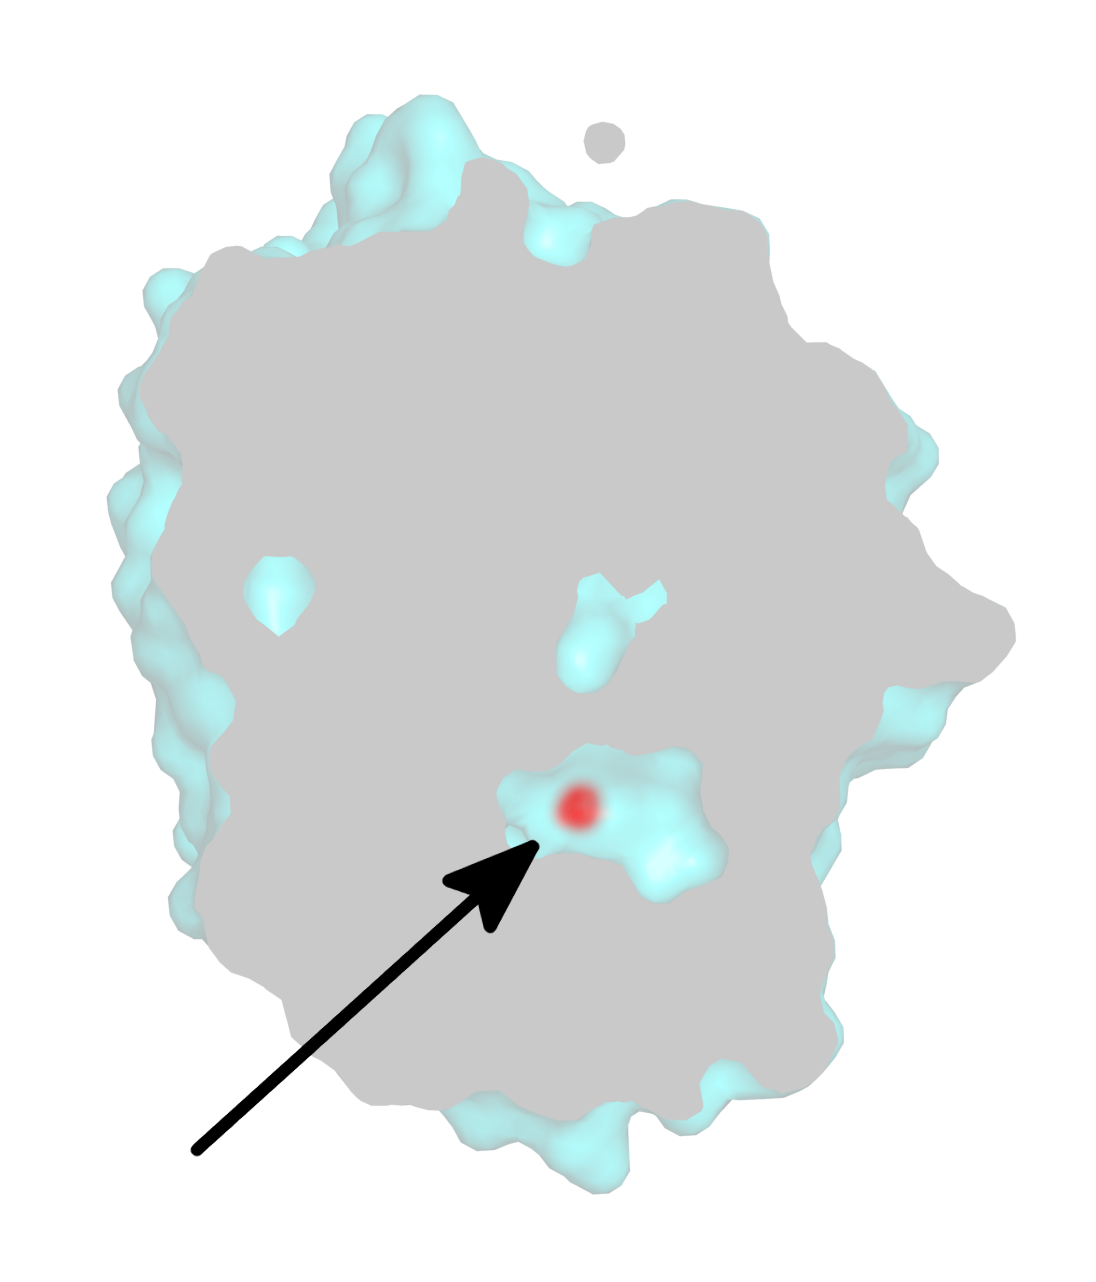
\includegraphics[width=0.25\textwidth]
{fig/motiv2lab} &
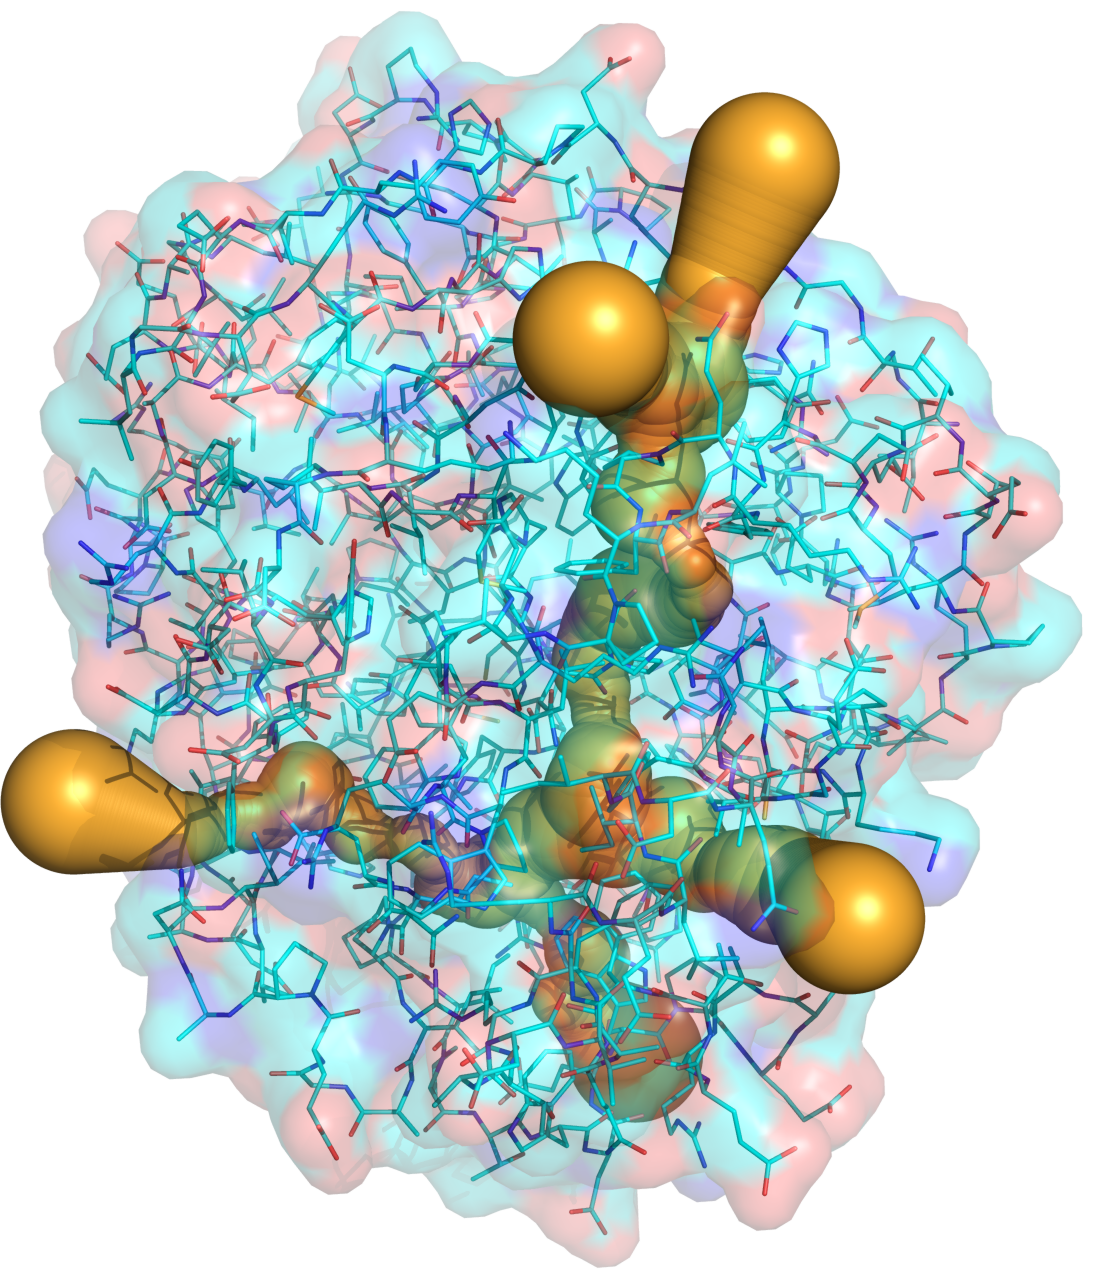
\includegraphics[width=0.24\textwidth]
{fig/motiv3}  \\
Protein  & Active site & Detected tunnels \\ %& Example of a  \\
             &            & (orange)         \\  %& trajectory
\multicolumn{3}{c}{%
\includegraphics[width=0.26\textwidth]
{fig/renderDCP.png}  \hskip 15pt
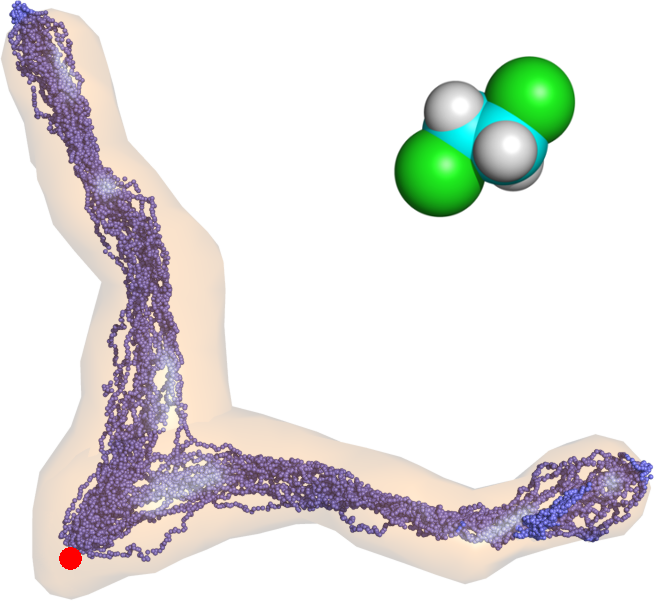
\includegraphics[width=0.24\textwidth]
{fig/render37t.png}} \\ 
\end{tabular}
}
\caption{\label{fig::motiv}
    \small
    Tunnels in the Haloalkane dehalogenase protein with possible trajectories of 1-Chlorpropan ligand (bottom left) and 1,2-Dichloroethane (bottom right).
}
\end{figure}

Our approach aims to overcome this problem by taking into account the actual shape of the ligand.
This necessarily requires to consider also conformational changes of the ligand, i.e., changes of the mutual position of the ligand atoms.
Such ligand is denoted as a flexible ligand.

The analysis of the traversability of tunnels by flexible ligands can be formulated as a motion planning problem and solved by sampling-based planners.
The sampling-based planners randomly sample the configuration space of the robot (ligand) and connect the collision-free samples into a graph structure (roadmap).
Rapidly Exploring Random Tree (RRT)~\cite{lavalleRRT} is one of the most used sampling-based planners. Besides many applications in robotics, the sampling-based planners have been already used in biochemistry as well, e.g., to study loop motions~\cite{cortes2004geometric}, to identify binding sites~\cite{bayazit2001ligand}, for exit pathway detection~\cite{cortes2010simulating,cortes2005path}, for tunnel detection~\cite{vonasek2017tunnel}, and especially for protein folding~\cite{raveh2009rapid,amato2002using}. %novinskaya2015improving

In this paper, we propose a modification of the RRT planner to find trajectories for non-spherical flexible ligands inside protein tunnels.
A tunnel is represented by a set of consecutive spheres surrounding the tunnel centerline.
Random samples are generated only around a given tunnel instead of the whole configuration space.
To enable the movement of the ligand in the narrow parts of the tunnel, the free-space is dilated by shrinking the atom radii, similarly, e.g., to~\cite{hsu06multilevel}.  %cortes2005path removed as it is not clear it they really rescale
The flexibility of the ligand is achieved by changing all or selected the dihedral angles.

Finding trajectories only along a given tunnel is faster than computing all possible exit paths, due to the decreased volume of the searched configuration space.
Another advantage of our method, in comparison with the existing approaches, is that we enable the users to trace the ligand path leading from the
outer solvent towards the protein active site.

The proposed method was tested by the biochemists who compared the results with already known trajectories of ligands, determined by their traditional approaches.
In the following section, we first mention several approaches and methods related to our solution and then describe the proposed method in detail.


\subsection*{Related Work}

{\color{red}BARA: vymezit se vuci Chexvis \cite{masood2015chexvis}}

Transportation of ligands into the protein active site can be directly evaluated using molecular dynamics (MD) simulations, where both the protein and ligand are flexible.
However, MD simulations are considerably computational demanding~\cite{kingsley2014including} and they have to be prepared
for a particular ligand/protein pair, which is not practical for testing a large number of different ligands interacting with the protein.
Therefore, computational approaches considering only geometry of ligand and proteins are still preferable due to their high speed.

The widely used approaches to evaluate the ligand traversability rely on the tunnel detection.
Most of the available tools for tunnel detection are based on Voronoi diagrams~\cite{yaffe2008,caver3,sehnal2013mole}.
Tunnels are represented as a sequence of spheres and characterized by their bottleneck, length, curvature, and the list of surrounding residues, whose physico-chemical properties are crucial for assessing of the feasibility of the protein-ligand interactions.
The tunnels are detected either on a single conformation of the protein, or, on a set of protein conformations, generated by MD simulations.
Computationally less demanding approaches for generating possible protein conformations are based on constrained geometric simulations, such as
ROCK~\cite{lei2004sampling}, FRODA~\cite{wells2005constrained}, and tCONCOORD~\cite{seeliger2007geometry}.
Examples of utilization of protein tunnels can be found in the recently published state-of-the-art report about the analysis and visualization of biomolecular cavities~\cite{Krone_2016}.

The main disadvantage of Voronoi diagram based tunnel detection methods is that the shape of the ligand is not taken into account during the tunnel detection.
Therefore, it is not easy to estimate if (and how) a non-spherical ligand can traverse the tunnel.
The ligand flexibility cannot be principally considered by Voronoi-based approaches and other techniques have to be adopted to solve this problem.

The traversability of a tunnel by a flexible ligand can be formulated as a motion planning problem and solved using the sampling-based motion planners.
These planners can cope with objects (robots) with many Degrees of Freedom (DOF) and they can also consider objects of an arbitrary shape.
Two widely used planners are the Probabilistic Roadmaps (PRM)~\cite{kavrakiForPP} and the Rapidly Exploring Random Tree (RRT)~\cite{lavalleRRT}.
The well known issue of the sampling-based planners is the narrow passage problem.
The narrow passage is a small region in the configuration space, whose removal changes the connectivity of the space.
Due to its low volume, the probability of sampling the narrow passage is low.
Consequently, many iterations are needed in order to put enough samples into the passages, which increases the computation time.
The PRM-based planners can cope with the narrow passage problem by increasing the probability of sampling in difficult regions, e.g., by sampling along the medial axis~\cite{wilmarthMAPRM}.
In~\cite{bergWIG}, the workspace is represented by a grid in which the difficult regions are identified using watershed labeling.
The regions can be estimated online, e.g., based on the number of collision-free samples around a given configuration~\cite{overmarsGauss,hsuBridge} or even identified by a human operator~\cite{denny2018general}. 

In the case of RRT-based planners, increasing the probability of sampling in difficult regions does not need to bring any advantage
if the growth of the tree is blocked by the obstacles.
To prevent this blocking, DD-RRT~\cite{yershovaDDRRT} limits the selection of nodes for the expansion to a small ball. 
The radius of this ball is set to infinity for new nodes, and decreases to a predefined radius if the node cannot be successfully expanded.
An automatic adaptation of this radius was proposed in the ADD-RRT~\cite{jailletADRRT}.
To attract the tree towards a given region, random samples have to be generated there only if the tree can expand to this region.
In~\cite{kardossRRTKK}, the probability of sampling is increased in several waypoints close to narrow passages, but without specifying how to find these waypoints.
The generalization of~\cite{kardossRRTKK} is the guided sampling, where a sequence of waypoints (a guiding path) is used to generate samples in the configuration space.
The guiding path can be computed in the workspace~\cite{vonasek2009rrt}, or iteratively refined in the configuration space based on the solution of a relaxed version of the problem~\cite{bayazitIRC}.

In the Retraction-based RRT~\cite{zhangRetraction}, the tree is retracted along the boundary of the obstacles in the configuration space.
The Selective Retraction-based RRT~\cite{lee2012srrrt} avoids the expensive growth in the open areas of the configuration space and focuses the retractions only on the narrow passages.
The Obstacle-based RRT~\cite{amatoOBRRT} utilizes several expansion procedures based on, e.g., random vectors, obstacle vectors, or medial axis.
In MARRT~\cite{denny2014marrt}, newly generated samples are pushed towards the medial axis.

The probability of sampling of the narrow passages can be increased by dilating the free-space, e.g., by shrinking the geometry of the robot or the obstacles~\cite{bayazitIRC}.

The shrinking technique has also been used in~\cite{cortes2010simulating}, where the exit pathways for a small flexible molecule are computed using a RRT-based method.
The flexible ligand is modeled as a kinematic chain, which increases the dimension of the configuration space.
To cope with these many-DOF ligands, the RRT-ML~\cite{cortes2007mlrrt} approach is employed as the basic planner in~\cite{cortes2010simulating}.
RRT-ML expands the tree primarily using those DOFs, that are essential for achieving the motion of the ligand (i.e., rotation
and translation) and it employs other DOFs (i.e., those that are responsible for conformational changes) if they hinder the growth of the tree.
In~\cite{singhLIG}, the pathways for a flexible ligand are found using PRM.
Each configuration in the roadmap is also evaluated using the electrostatic energy.
The high-energy configurations are discarded, while the low-energy configurations (and their vicinity) are sampled densely.
The approach~\cite{singhLIG} can also predict the ligand binding sites.





\subsection*{Contributions}
{\color{red}Rewritten, please check. VV: I suggest to rewrite this after we describe experiments. I will take care of it }

We propose a utilization of sampling-based motion planning to compute trajectories of flexible ligands in the protein tunnels.
The input of the proposed method is a set of tunnels computed using Voronoi diagrams.
The method computes feasible trajectories for a given ligand along the given tunnels. 
The trajectories can be computed both from the surface of the protein to the active sice or vice versa.

%The tunnels are detected on selected protein conformations, resulting, e.g., from MD simulations or from a tool providing the protein conformation sampling~\cite{lei2004sampling,wells2005constrained,seeliger2007geometry}.

In contrast to~\cite{cortes2010simulating}, which searches for any exit pathway from the protein, we localize the searching and compute the trajectories only along each tunnel separately, which allows the biochemists to analyze selected tunnels.
Computing the trajectories along a single tunnel brings several advantages from the motion planning point of view as well.
The random samples are not generated in the whole configuration space, but only around the tunnel in a user-defined distance. 
This helps to cope with the narrow passage problem.
By selecting a tunnel to be analyzed, the users help the planner to focus only on a subset of the whole configuration
space, similarly as in~\cite{denny2018general}.
Consequently, the volume of the configuration space to be searched is decreased, while the relative volume of the narrow passages is increased.

It has been observed, that the tunnels detected in protein conformations without ligands (provided by MD simulations without ligands or by
protein conformation sampling) are rather narrow. 
However, MD simulations of proteins with ligands have shown that the tunnels can move, merge and adapt to the shape of the passing ligand and vice versa.
In consequence, even very narrow tunnels, being too small for the passage of a given ligand-approximating sphere, can potentially serve as the transportation path for the ligand.
Therefore, also the existing Voronoi-based methods enable the user to decrease the size of the approximating sphere which simulates the shrinking of the ligand size.
In our solution, we simulate this by shrinking the atom radii of the ligand, which is used also by~\cite{cortes2010simulating,guieysse2008structure}.

%MD simulations of ligands passing through proteins show that the ligands can be highly flexible.
%All possible conformations of a ligand are determined by the torsion and dihedral angles between its atoms, but the low-energy conformations are preferred.
%Therefore, the ligand flexibility can be modeled using only a predefined set of low-energy conformations.
%By using the set of predefined conformations, it is not necessary to model the additional degrees of freedom, so 
%the dimension of the configuration space is not increased as in~\cite{cortes2010simulating}.
%



\section*{Methods}

\subsection*{Preliminaries}

Proteins and ligands are represented by the hard sphere model, where each atom is represented by a sphere and whose radius 
is the van der Waals radius.
The flexibility of the ligand is modeled as an articulated kinematic chain with $m$ joints.
The joints are determined by the rotatable bonds of the ligand which is described by the PDBQT~\cite{pdbqt} format.

A configuration $q=(x,y,z,r_x,r_y,r_z, \alpha_1,\ldots,\alpha_m)$ of the ligand describes its 3D 
position $(x,y,z)$, 3D rotation $(r_x,r_y,r_z)$ and $m$ internal degrees of freedom $\alpha_i$ modeling  the rotatable bonds.
All configurations form the configuration space $\C$.
The configurations, where the ligand does not collide with the protein, form the subset $\CF \subseteq \C$.
Therefore, the task of finding the trajectory of the ligand can be solved by finding a path from the
start configuration $\qstart \in \CF$ towards the goal $\qgoal \in \CF$.
The distance $\dist(q_a,q_b)$ between two conifguration $q_a$ and $q_b$ is measured by the 6D Euclidean metric using
both translation and rotation part of the two configurations.
Let $\distt(c,q)$, $c \in \R^3, q \in \C$ denote 3D Euclidean distance between the 3D point $c$ and
the translational part of the configuration $q$.

A protein tunnel is described by a sequence of $n$ collision-free spheres $T=( (c_i, r_i) )$, $i=1,\ldots,n$, 
where $c_i \in$ $\mathbb{R}^3$ is the center and $r_i > 0$ is the radius of the $i$-th spehere.
The tunnels can be computed using any existing tool, e.g., CAVER 3.0~\cite{caver3}, or CHEXVIS~\cite{masood2015chexvis}.

Collision detection between the atoms of the ligand and the atoms of the protein is used
to determine collision-free samples.
Fast collision detection can be realized using hierarchical methods such as bounding volume hiearchy~\cite{ericson2004real}.
In the case of protein/ligand interactions, it is common to enable little penetration between the ligand's and 
the protein's atoms~\cite{cortes2010simulating}, which can be achieved by a slight decrease
of the atom radii, e.g. to the 80~\% of the original value, which is also considered in this paper.


\subsection*{Computing Ligand's trajectories using Sampling-based Planning}

The proposed method utilize the RRT principle~\cite{lavalleRRT} to search the configuration space.
The RRT method builds a tree $\T$ of collision-free configurations rooted in $\qinit \in \CF$, which is expanded
towards the random samples generated uniformly in the configuration space $\C$.
Finding ligand trajectories in the tunnels requires to steer the growth of the tree from the start of the tunnel to its end.
This is achieved by generating the random samples progresivelly along the tunnel.
Let $1 \le v \le n$ denote the index of a sphere $c_v$ of the tunnel, we denote to this sphere as to the active sphere in the rest of the paper.
The random sample $\qrand$ is generated around  $c_v$ with probability $\gb$; otherwise, it is generated uniformly in $\C$.
To generate the random sampla around the active sphere $c_v$, the 3D position of $\qrand$ is generated from $N(c_i,\Sigma)$, where
$\Sigma$ is the $3\times 3$ diagonal matrix with value $r_v$ on the diagonal.
The rotational part of $\qrand$ is generated uniformly, i.e., $r_x,r_y,r_z \sim U(-\pi,\pi)$ and the internal degrees of 
freedom $\alpha_i=0$, $i=1,\ldots,m$.

The main loop of the proposed method is listed in Alg.~\ref{alg::main}.
At the begining, the tree $\T$ is initialized with the start configuration $\qinit \in \CF$ and the active sphere
is set to the begining of the tunnel, $v=1$.
In each iteration, a random sample $\qrand$ is generated as describe above.
The nearest node $\qnear \in \T$ towards $\qrand$  in the tree is found and expanded.
The task of the expansion is to find a new configuration $\qnew$ around $\qnear$ that minimizes the distance
towards $\qrand$.
The vicinity of $\qnear$ is sampled by $k$ random samples $\qnew'$. 
The translational part of $\qnew'$ is generated from $N(pos(\qnear),\Sigma')$, 
where $pos(\qnear)$ is the translational part of $\qnear$ and $\Sigma'$ is
the $3 \times 3$ diagonal matrix with values $\varepsilon$ on the diagonal, and $\varepsilon$ is the resolution of the planner.
The rotational part of $\qnew'$ is generated from $N(rot(\qnear), \Sigma_r)$, where $\Sigma_r$ is the $3 \times 3$ diagonal
matrix with values $\pi/3$ and the internal degrees of freedom $\alpha_i$ of $\qnew'$ are generated
randomly from $U(-\pi,\pi)$.
Each sample $\qnew'$ is checked for collision and the from the collision-free one samples, the nearest towards $\qrand$ is 
selected, which results in a new configuration $\qnew$.
The resulting configuration is then added to the tree and the node $\qnear$ is marked as the parent of the node $\qnew$.
During the expansion (Alg.~\ref{alg::expand}), the vicinity of $\qnear$ is sampled with $N$ predefined
samples.
The samples are tested for collisions and the collision-free samples, that minimize the distance to $\qrand$ are added to the tree.

After the sucessful expansion, the distance to the center of the active sphere is calculated.
If the tree approaches the active sphere to the predefined distance $\dtg$, new active sphere of the tunnel is determined.
The distance $\distt(c_i, q'), i=v+1,\ldots,n$ between each subsequent sphere and it's nearest node in the tree $q' \in \T$ 
is calculated. 
The sphere with the lowest index $i$ whose distance towards the tree is larger than $\dtg$ is set as the active sphere.
Setting the virtual goal to this successor allows the tree to avoid such parts of the tunnels that are not traversable or reachable by the ligand.
The tree can slightly detour from the tunnel and overcome difficult parts (e.g., the tunnel bottleneck) by finding an alternative trajectory nearby.

The parameter $\dtg$ determines how far can the tree detour from the tunnel centerline.
In case of tunnels not having other tunnels in the close vicinity (which is very common), we recommend using the double value of the tunnel average width.
The algorithm terminates after a predefined number of planning trials $\Imax$ or if the tree reaches
the last sphere in the tunnel, i.e., when $v = n$.

\linesnumbered
\begin{algorithm}[b]
{\small
\setstretch{0.88}
\caption{\label{alg::main}Trajectory planner}
\KwIn{
    tunnel $T=( (c_i, r_i) )$, $i=1,\ldots,n$, with spheres centers $c_i \in \R^3$ and radii $r_i$,
    initial configuration $\qinit$
}
\KwData{
   distance $\dtg$ to move virtual goal,
   tunnel bias $\gb$
}
\KwOut{
    configuration tree $\T$\;
}
\hrule
$v = 1$; // index of the virtual goal\\
$iteration = 0$\;
$\T$.addNode($\qinit$)\;
\While{$iteration < \Imax$ {\bf and}  $v < n$}{
    \eIf{$rand() < \gb$}{
        $\qrand$ = random sample around virtual goal $c_v\!\in\!T$; \nllabel{main::s1} \\
    }{
        $\qrand$ = random sample from $\C$; \nllabel{main::s2} \\
    }
    $\qnear$ = nearest node in $\T$ towards $\qrand$\;
    expand($\T, \qnear,\qrand$)\;
    \For{$i=v,v+1,\ldots,n$}{ \nllabel{alg::main:a}
        $q'$=$\T$.nearestNode($c_i$)\;
        \If{$\distt(c_i,q') > \dtg $}{
            $v = i+1$; // new virtual goal found\;
            {\bf  break}\;
        }
    } \nllabel{alg::main:b}
    \If{$v=n+1$}{
        // last sphere of the tunnel is reached
        return $\T$.reconstructPath($\qinit,\qnew$)\;
    }
    $iteration = iteration+1$\;
}
\return $\T$\;
}
\end{algorithm}

To generate the samples $\qrand$ around the virtual goal $v$, the translation part $(x,y,z)$ of $\qrand$ is generated
from the Gaussian distribution $N(c_v,\Sigma)$, where $\Sigma$ is the diagonal matrix with diagonal entries equal to the parameter $\rv$, 
and the rotational part of $\qrand$ is generated using techniques described in~\cite{kuffnerES}.
The ligand index $l$ and scale $s$ can be set to zero, as these are not used in the employed metric for the nearest-neighbor search.
The parameter $\rv$ influences the distribution of the random samples around the tunnel centerline. 
We propose to set this parameter to the average width of the tunnel.

\begin{algorithm}[b]
{\small
\setstretch{0.88}
\caption{\label{alg::expand}expand}
\KwIn{
   tree $\T$,
   configuration $\qnear$ to be expanded,
   random configuration $\qrand$
}
\KwData{
   number of trials $k$
}
\hrule

$\qnew = \emptyset$; // empty configuration \nllabel{alg::expa} \\
\For{$i = 1,\ldots,k$}{
    $q=\qnear$\;
    $q.position$ = random 3D position around $\qnear$\;
    $q.rotation$ = random 3D rotation\;
    \If{isCollisionFree($q$)}{
        \If{$\qnew = \emptyset$ {\bf or} $\dist(q, \qrand) < \dist(\qnew,\qrand)$}{ \nllabel{alg::expand:a}
            $\qnew = q$\;
        }
    } 
}
\nllabel{alg::expb}
\If{$\qnew \ne \emptyset$} {
    $\T$.addNode($\qnew$)\;
    $\T$.addEdge($\qnear,\qnew$)\;
    {\bf break;} // go to the next conformation
}
}
\end{algorithm}

The result of each planning trial is the tree $\T$ of collision-free configurations in which a path
between $\qinit$ (root of the tree) and $q'$ is found, where
 $q'$ is the nearest node to the end of the tunnel (measured using the 3D Euclidean metric). 



\section*{Results and Discussion}
\subsection*{Experimental Verification}

The proposed algorithm was verified in two scenarios: on a sequence of frames of MD simulation and on a set of protein conformations 
provided by the conformation sampling approach.

\subsubsection*{Analysis of MD simulation}

\paragraph*{Algorithm and data setup}
The task is to compute the ligand traversability towards the active site using two main tunnels in the Haloalkane dehalogenase protein (DhaAwt, PDB ID 4E46), which consists of 4650 atoms.
The MD simulation was computed using AMBER~12 (details about the used MD simulations of DhaAwt/4E46 are described in~\cite{marques2017catalytic}).
The tunnels were detected in 100 consecutive frames of MD simulation in the part where the protein was already stabilized.
The tunnels for the probe 0.9~\AA\ towards the active site defined by residues 38 (Asparagine), 102 (Histidine), and 103 (Aspartic Acid) were
computed using the CAVER 3.0~\cite{caver3} tool.
In most of the frames, two tunnels were detected.
The average bottleneck sizes of these tunnels were $1.48$~\AA\ and $1.2$~\AA\ for the main and side tunnel, respectively.

Models  of the ligands in Mol2 formats were converted to the param files~\cite{meiler2006rosettaligand}, containing the topology, rotatable bonds, atom types, and partial charges. 

The methods \RA\ and \RB\ differ in the expansion step (lines \ref{alg::expa}--\ref{alg::expb} in Alg.~\ref{alg::expand}).
In these lines, the \RB\ method employs the retraction step in order to find a new collision-free configuration $\qnew$ that approaches $\qrand$.
The retraction step is realized by sampling the vicinity of the configuration $\qnear$ in the distance $0.05$~\AA\ using 20 samples.
A collision-free sample that maximally approaches $\qrand$ is selected and added to the tree, and the retraction continues from this sample.
The retraction step is repeated 5 times.
The \RB\ method can therefore expand the tree by at most 5 new nodes per ligand conformation, while \RA\ extends the tree only by one new node.
The larger number of nodes in \RB\ method is not problematic, as the KD-trees were used for the nearest-neighbor search and the time to solve these queries is significantly smaller than the collision detection.
The parameters of the methods were selected in such a way that the number of collision detection queries in each expansion step is the same.
For each conformation and tested scale, the \RA\ method checks $m=100$ candidate configurations for collision, and \RB\ checks $5 \times 20$ configurations for collision.
Other parameters of the \RB\ planner were the same as for \RA.
The planning was terminated after $\Imax$ iterations or if the tree approached the active site to the distance less than 2~\AA\ (i.e., the 
geometric center of the ligand was closer than 2~\AA\ from the active site).

The performance of the methods is evaluated using the traversability rate, which is the percentage of frames of the protein dynamics that are traversable by the tested ligand.
This distance is measured as the 3D distance between the geometric center of the ligand and the position of the active site.


%\paragraph*{Influence of the Conformation Selection}
%The number of generated ligand conformations $|\L|$ depends on the number of rotatable bonds of the ligands and even though only
%the low-energy conformations are stored in $\L$, the set can still contain thousands of conformations.
%For fast motion planning we utilize a subset of the original set $\L$.
%The aim of this experiment was to verify the proposed selection of ligand conformations from a large set $\L$ (Sec.~\ref{sec::strat}).
%
%Two selection strategies were tested:
%the strategy described in Sec.~\ref{sec::strat} (denoted `S') and the strategy that prefers smaller (packed) conformations (denoted `P').
%The `P' method selects such conformations where the deviations of the atomic distance from the geometric center are the lowest, which leads 
%to the selection of packed conformations.
%The strategies were tested using the ligand DCP (Dichloropropanol), for which  $|\L|=1300$ conformations were created, and for the ligand
%m040 (1,5-Dichloropentane) with $|\L|=7560$ conformations.
%
%The traversability rates are shown in Tab.~\ref{tab::selection}, where the subscript of each ligand's 
%name shows the number of the selected conformations (5 or 50) and the used method (S or P).
%In case of both tested ligands and 50 selected conformations, the `S' strategy leads to a higher traversability rate than the `P' strategy.
%For the DCP ligand, the higher traversability rate was achieved when 50 conformations were selected.
%This experiment shows that selecting 50 conformations using the `S' strategy (Sec.~\ref{sec::strat}) leads to better results
%than using the smaller number of conformations or when preferring the packed conformations.
%
%\begin{table}[bt]
%\centering
%\caption{\label{tab::selection}
%    \small
%    The influence of the conformation selection method on the traversability rates in the first (main) tunnel of the 4E46 protein.
%    The number after~`$/$' denotes the number of atoms.
%}
%\small
%\renewcommand{\tabcolsep}{4.3pt}
%{\scriptsize
%\input graphSelNew.tex
%}
%\end{table}



\paragraph*{Traversability of Ligands}
Based on the results of the previous experiment, 
      %50 conformations using the `S' strategy (Sec.~\ref{sec::strat})  were selected for 
      ligands 
m037t (1,2-Dichloroethane), m038t (1,3-Dichloropropane), m056 (2-Chlorobutane), and m080 (Trichloropropane).

\begin{table}[bt]
\centering
\caption{\label{tab::main}
    \small
    Traversability rate over 100 frames for ligands with 50 conformations in the 4E46 protein.
    The number after '$/$' denotes the number of atoms.
}
\small
\renewcommand{\tabcolsep}{2pt}
{
\scriptsize
%\input graphNewNoA3.tex %without \rc (a1*) column
}
\end{table}

The traversability rate is shown in Tab.~\ref{tab::main}. 
Only the traversability of the main tunnel is shown, as no trajectory was found in the side tunnel for most of the tested ligands.
The only exception is the ligand m037t, which was the smallest tested one (consisting of 8 atoms), and therefore it could fit even inside the side tunnel.
The traversability rate is higher for the most scaled-down ligands  and it decreases with the increasing scale.
For the DCP ligand, the trajectories were detected in 18~\% of frames for scale and the traversability of this ligand
to the active site was approved by a separate MD simulation~\cite{marques2017catalytic}.
Based on the success rate, also other ligands (e.g., m037t with traversability rate 45~\% at $smin$=0.8) seem to be promising.
However, their binding was not yet approved by dedicated MD simulations.
The planning was realized with 50 conformations of the ligands, but not all of them were used, which is shown in Tab.~\ref{tab::m040c}.

Besides scaling-down the ligand, also the atoms of the protein can be scaled, which is used, e.g., in~\cite{cortes2005path}, where the scale 0.8 is used for both the ligand and protein.
We tested also this option using \RA\ (the column \RD\ in Tab.~\ref{tab::main}).
The results are similar to the results of \RA\ and $smin=0.6$ (except for DCP and m040, which can be a result of randomization).

The proposed \RA\ planner provides higher traversability rate than the RRT-Retraction (\RB).
The distances of the configuration trees (measured using the 3D Euclidean metric) to the active site and the runtimes in each frame
are shown in Fig.~\ref{fig::comparison}.
The runtimes of \RB\ are higher than the runtimes of \RA\ and the standard deviations as well.

\begin{table}[t]
\caption{\label{tab::m040c}
\small
Examples of elongated/packed conformation for m040 (1,5-Dichloropentane).
The table shows the average number of different ligand conformations (out of 50) used in trajectories reaching the active site in the 4E46 protein.
}
\centering
{\footnotesize
%\def\arraystretch{0.9}
\begin{tabular}{cc}
\rotatebox{0}{\hskip 5pt Long} \\ 
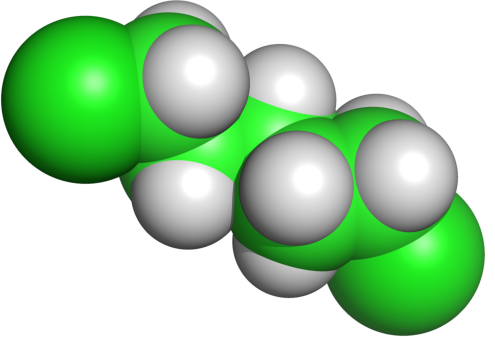
\includegraphics[width=0.07\textwidth]
{fig/m040-conf1} \\
\rotatebox{0}{Packed} \\ 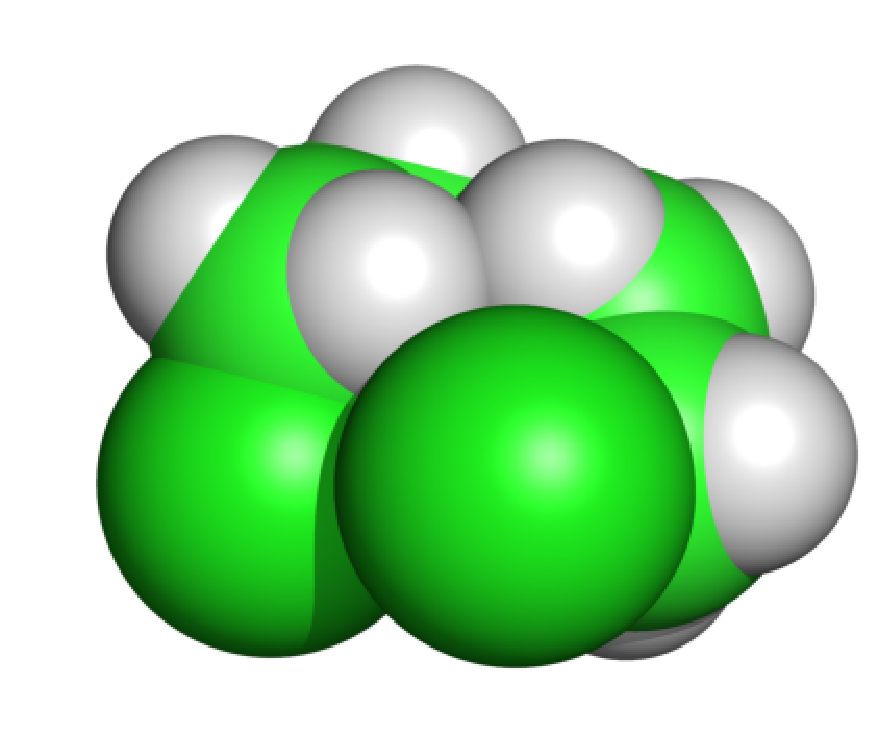
\includegraphics[width=0.055\textwidth]
{fig/m040-conf2}
\end{tabular}
}
{\scriptsize
\def\arraystretch{0.9}
%\input usedc.tex
}
\end{table}

\subsubsection*{Analysis of Protein Conformations}
The task of the second analysis was to find the trajectory for the ligand 4-(4-benzylphenyl)-1,3-thiazol-2-amine into the active
site of A4 hydrolase (PDB ID 4L2L, 9666 atoms).
The tCONCOORD tool~\cite{seeliger2007geometry} was used to generate 1000 conformations of the protein 4L2L.
The initial PDB structure was minimized by GROMACS 4.0.7 using the input parameters recommended on the example page of tCONCOORD~\cite{tconcoord}.
The protein conformations were generated using the default settings for tCONCOORD in the PERT mode. % which only perturbs the starting configuration of atoms instead 
The tunnels leading to the active site defined by residues 134 (Alanine) and 311 (Phenylalanine) were computed by CAVER 3.0, using the probe 0.9~\AA.
All 1000 conformations contained at least 5 tunnels. % more than 900 conformations contained 9 tunnels.
The ordering of the detected tunnels slightly differs in different conformations.
Therefore, the first three widest tunnels were used (with average bottlenecks 1.22~\AA, 1.20~\AA\, and 1.19~\AA\ with the average lengths 22.3~\AA, 25.3~\AA\, and 28.4~\AA, respectively).
20 starting configurations were found at the begining of each tunnel, and 10 trajectories were computed for each starting configuration.
The conformations of the ligand were prepared in the same way as in the previous section.
From the available $|\L|=736$ low-energy conformations, 100 were selected using the `S' strategy.

\begin{table}[bt]
\centering
\caption{\label{tab::4l2l}
    \small
    Traversability rate in 1000 conformations of the protein 4L2L in the first three tunnels.
}
\small
\renewcommand{\tabcolsep}{2pt}
{
\scriptsize
%\input traversability.tex
}
\end{table}

As the tested ligand is a known inhibitor of the protein 4L2L~\cite{marques2017enzyme} we assumed that the ligand can reach the active site.
Due to large size of the ligand (33 atoms), low scale-down factors $smin\in\{0.4,0.5,0.6\}$ were used and
the active site was considered as reached if the distance to the geometric center of the ligand was less than 5~\AA.
All parameters of the \RA\ were set as in the previous experiment, except $\Imax=100\cdot10^3$.
The proposed planner was able to find trajectories even for this large ligand inside the long tunnels, which is
shown by the traversability rates (Tab.~\ref{tab::4l2l}).
Example of the solution is depicted in Fig.~\ref{fig::inhibitor}.

\begin{figure}
\centering
\vskip -5pt
\includegraphics[width=0.8\textwidth]{fig/4l2l-solution.png}
\caption{\small
    \label{fig::inhibitor}Example of a found trajectory inside the tunnel No. 1 of the 4L2L protein with the final position of the ligand.
}
\end{figure}


\subsection*{Discussion and Utilization of the Results}
The presented work is motivated by the current needs of biochemists who need to analyze the traversability of selected ligands through selected protein tunnels.
Due to the low bottleneck of tunnels, it is often required to shrink the atomic radii of the ligand, as utilized also in other existing tools.
Finding trajectories for the scaled-down ligands enables to solve the problem with narrow passages, but it can be questionable how biochemically relevant such trajectories~are.

Determination of the proper scaling-down factor requires long-term testing of many exemplary simulations and needs to be performed by the biochemists. 
Therefore, it is beyond the scope of this paper, which focuses namely on the algorithmic part of the problem.
The scales used at the trajectory points can provide the biochemists with new knowledge about the ligand behavior, which was impossible to get using the Voronoi-based approaches.
Judging the accessibility of the active site by a ligand based only on the traversability rates may be problematic if the ligand is scaled down too much.
The visualization of the computed trajectories can show those parts of the tunnel where the ligand had to be scaled-down significantly (red parts of trajectories in Fig.~\ref{fig::dcp}), and parts where the ligand could be enlarged again (green parts in Fig.~\ref{fig::dcp}).

According to the results of the motion planning, the DCP ligand needs to shrink down to approximately 75~\% of its size, but only at one part of the tunnel (Fig.~\ref{fig::dcp}, point B). 
Beyond this point, the ligand can move at larger scales again.
As both the protein and ligand mutually influence each other, it is possible that even such a narrow part of the tunnel is traversable.
This was observed in a separate MD simulation of the DCP ligand in the 4E46 protein, which revealed that DCP can pass the main tunnel~\cite{marques2017catalytic}. 
The necessity to scaled-down even more than 0.8, which is a value used by other tools~\cite{cortes2010simulating}, was
shown also in the second experiment, where the trajectory for the inhibitor of the 4L2L protein required scaling down to 0.5 or 0.6.

{\def\a{0}
\begin{figure}[t]
\centering
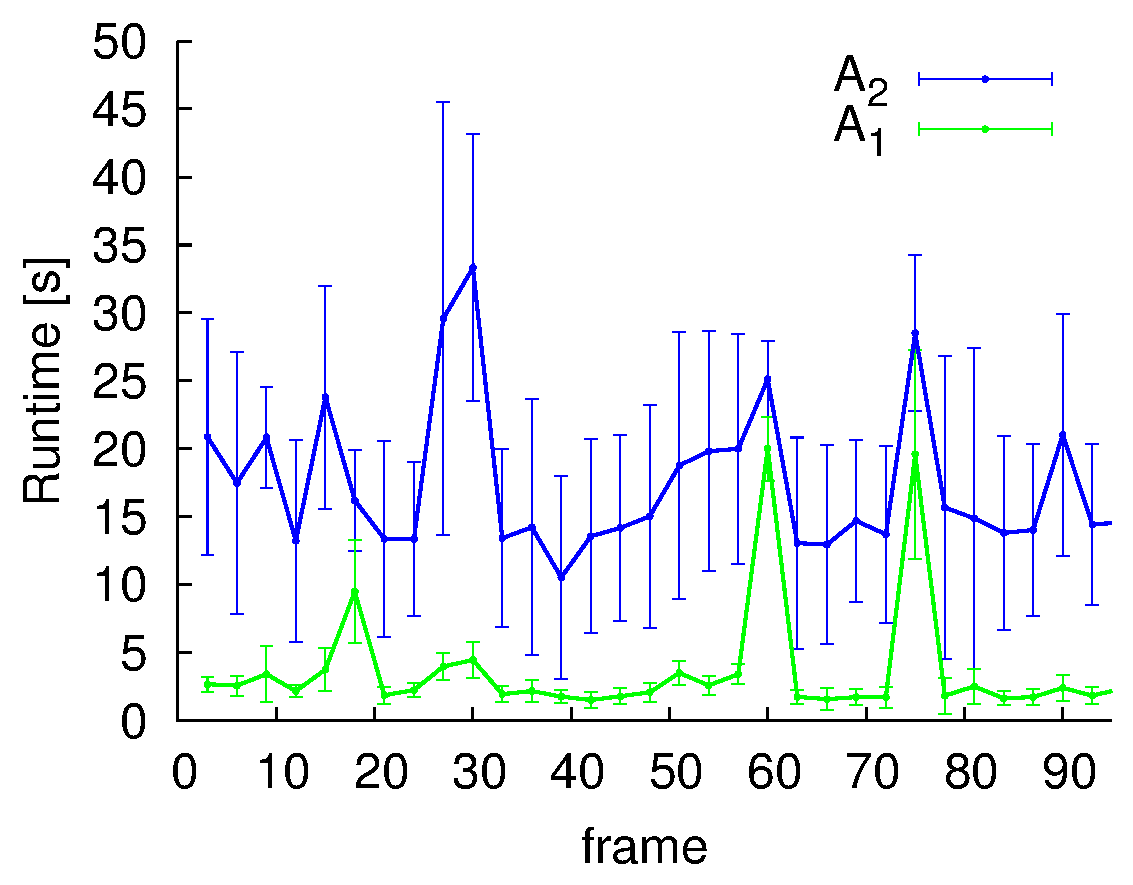
\includegraphics[width=0.44\textwidth,angle=\a]{fig/crop3}
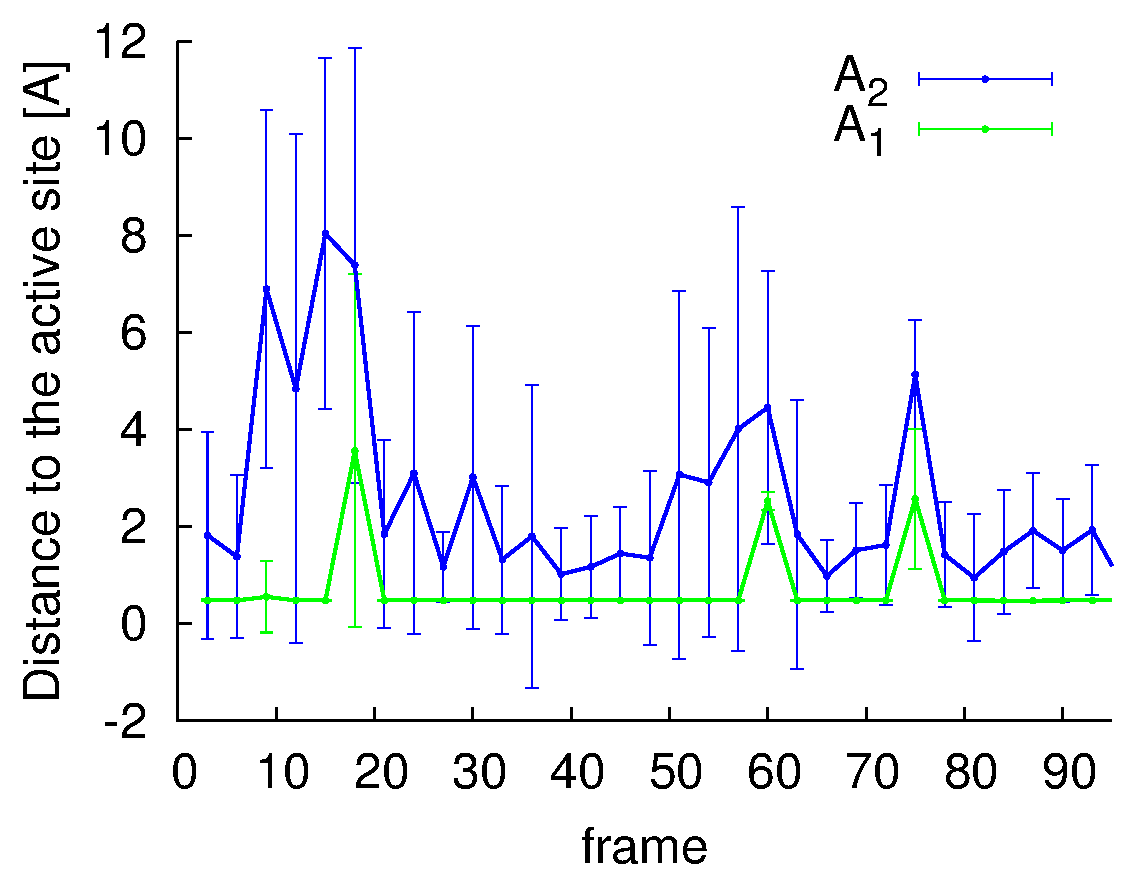
\includegraphics[width=0.44\textwidth,angle=\a]{fig/crop4}
\caption{\label{fig::comparison}
    \small
    Runtimes and the distance to the active site for the m037 ligand at scale 0.7.
    The values are computed from all 200 trials (20 initial configurations $\times$ 10 trials).
    Only each third frame is shown in the graph.
}
\end{figure}
}

\begin{figure}
\centering
\vskip -5pt
\includegraphics[width=0.8\textwidth]{fig/dcp-image1Label}\\
\vspace{-5pt}
\caption{\label{fig::dcp}
    \small
Visualization of trajectories for the ligand DCP in the two examined tunnels.  
The color of the trajectories corresponds to the scale, that was needed to pass the given part of the tunnel.
The ligand can enter the first tunnel with a high scale (almost 1=100~\%) (A), but then it has to be scaled-down (to $\sim75$~\%) to pass the
next part of the tunnel (B). After this narrow passage, the tunnel is larger again and the ligand can traverse to the narrow passage with
scale $>75$~\% (C).
The second tunnel can also be entered with the high scale (green), but then the narrow part is traversable only with a low scale ($\sim50$~\%) (D). 
For the visualization purposes, even more scale-down to 0.3=30~\% was allowed (E) to see how the ligand passed the tunnel.
The ligand can reach the active site only at a very low scale ($\sim0.4=40$~\%) using the side tunnel.
}
\end{figure}

\subsection*{Conclusion}
We presented a novel modification of the RRT planner to compute trajectories of ligands inside selected protein tunnels.
The ligand shape is taken into account and the ligand flexibility is modeled using a predefined set of its conformations.
The ligand conformations are prepared using the Rosetta tool, ranked by their energy and only low-energy conformations are used in the planning.
To simulate the real behavior of ligand passing through the tunnel, we enable scaling down the atomic radii of the ligand up to a certain predefined factor.
The planner generates the random samples only along a tunnel computed by the Voronoi diagram, and it attempts to expand the configuration
tree using all ligand conformations. 
The expansion prefers atoms with a higher scale, which ensures that the ligand shrinks down only if necessary, i.e., when traversing the narrow parts of the tunnel.

%%%%%%%%%%%%%%%%%%%%%%%%%%%%%%%%%%%%%%%%%%%%%%
%%                                          %%
%% Backmatter begins here                   %%
%%                                          %%
%%%%%%%%%%%%%%%%%%%%%%%%%%%%%%%%%%%%%%%%%%%%%%

\begin{backmatter}

\section*{Competing interests}
  The authors declare that they have no competing interests.

\section*{Author's contributions}
    Text for this section \ldots

\section*{Acknowledgements}
The presented work has been supported by the Czech Science Foundation (GA{\v C}R) under research project No. 17-07690S.

%%%%%%%%%%%%%%%%%%%%%%%%%%%%%%%%%%%%%%%%%%%%%%%%%%%%%%%%%%%%%
%%                  The Bibliography                       %%
%%                                                         %%
%%  Bmc_mathpys.bst  will be used to                       %%
%%  create a .BBL file for submission.                     %%
%%  After submission of the .TEX file,                     %%
%%  you will be prompted to submit your .BBL file.         %%
%%                                                         %%
%%                                                         %%
%%  Note that the displayed Bibliography will not          %%
%%  necessarily be rendered by Latex exactly as specified  %%
%%  in the online Instructions for Authors.                %%
%%                                                         %%
%%%%%%%%%%%%%%%%%%%%%%%%%%%%%%%%%%%%%%%%%%%%%%%%%%%%%%%%%%%%%

% if your bibliography is in bibtex format, use those commands:
\bibliographystyle{bmc-mathphys} % Style BST file (bmc-mathphys, vancouver, spbasic).
\bibliography{paper}      % Bibliography file (usually '*.bib' )
% for author-year bibliography (bmc-mathphys or spbasic)
% a) write to bib file (bmc-mathphys only)
% @settings{label, options="nameyear"}
% b) uncomment next line
%\nocite{label}

% or include bibliography directly:
% \begin{thebibliography}
% \bibitem{b1}
% \end{thebibliography}

%%%%%%%%%%%%%%%%%%%%%%%%%%%%%%%%%%%
%%                               %%
%% Figures                       %%
%%                               %%
%% NB: this is for captions and  %%
%% Titles. All graphics must be  %%
%% submitted separately and NOT  %%
%% included in the Tex document  %%
%%                               %%
%%%%%%%%%%%%%%%%%%%%%%%%%%%%%%%%%%%

%%
%% Do not use \listoffigures as most will included as separate files

\section*{Figures}
%  \begin{figure}[h!]
%  \caption{\csentence{Sample figure title.}
%      A short description of the figure content
%      should go here.}
%      \end{figure}

%\begin{figure}[h!]
%  \caption{\csentence{Sample figure title.}
%      Figure legend text.}
%      \end{figure}

%%%%%%%%%%%%%%%%%%%%%%%%%%%%%%%%%%%
%%                               %%
%% Tables                        %%
%%                               %%
%%%%%%%%%%%%%%%%%%%%%%%%%%%%%%%%%%%

%% Use of \listoftables is discouraged.
%%
%\section*{Tables}
%\begin{table}[h!]
%\caption{Sample table title. This is where the description of the table should go.}
%      \begin{tabular}{cccc}
%        \hline
%           & B1  &B2   & B3\\ \hline
%        A1 & 0.1 & 0.2 & 0.3\\
%        A2 & ... & ..  & .\\
%        A3 & ..  & .   & .\\ \hline
%      \end{tabular}
%\end{table}

%%%%%%%%%%%%%%%%%%%%%%%%%%%%%%%%%%%
%%                               %%
%% Additional Files              %%
%%                               %%
%%%%%%%%%%%%%%%%%%%%%%%%%%%%%%%%%%%

%\section*{Additional Files}
%  \subsection*{Additional file 1 --- Sample additional file title}
%    Additional file descriptions text (including details of how to
%    view the file, if it is in a non-standard format or the file extension).  This might
%    refer to a multi-page table or a figure.

%  \subsection*{Additional file 2 --- Sample additional file title}
%    Additional file descriptions text.


\end{backmatter}
\end{document}
